\documentclass[answers]{exam}

% \documentclass[addpoints]{exam}

\usepackage{xeCJK}
\usepackage[utf8]{inputenc}
\usepackage{graphicx}
\usepackage{hyperref}
\usepackage{amsmath}
\usepackage{booktabs}
\usepackage{wrapfig}
    
\pagestyle{headandfoot}
\firstpageheadrule
\firstpageheader{\textbf{Okayama University}}{\textbf{WANG JING}}{\textbf{Superconductivity Final Exam}}
\runningheader{Okayama University}
{}
{Superconductivity Final Exam}
\runningheadrule
\firstpagefooter{}{Page \quad\thepage\ }{}
\runningfooter{}{Page\quad\thepage\ }{}

% no box for solutions
% \unframedsolutions

\setlength\linefillheight{.5in}

\renewcommand{\solutiontitle}{\noindent\textbf{Answer:}}
% \renewcommand{\solutiontitle}{\noindent\textbf{解:}\par\noindent}

\renewcommand{\questionlabel}{\thequestion .}
\renewcommand{\thepartno}{\arabic{partno}}
\renewcommand{\partlabel}{\thepartno .}


\begin{document}
\textbf{I. A two-dimensional free-electron gas.}
\begin{questions}
\question Using the 2-dimensional Schr\"odinger equation, show that the wave function and energy band are :
\begin{gather*}
\psi_{\vec{k}}(\vec{x}) =B \mathrm{e}^{i k_{x} x} \mathrm{e}^{i k_{y} y}\notag \\
E_{\vec{k}} =\frac{\hbar^{2}\left(k_{x}^{2}+k_{y}^{2}\right)}{2 m}\notag   
\end{gather*}
where $m$ is the mass of the electron, $\vec{k} = (k_{x}, k_{y})$ is the wave vector and $B$ is the normalization constant.
\begin{solution}
For  2-D  shr\"odinger Equation:
\begin{align*}
-\frac{\hbar^{2}}{2 m} \nabla^{2} \psi(\vec{r})+V \psi(\vec{r})=E \psi(\vec{r})
\end{align*}
With  V=0 
\begin{align*}
-\frac{\hbar^{2}}{2 m} \nabla^{2} \psi(\vec{r})=E \psi(\vec{r})
\end{align*}
The solution of this equation is travelling plane wave:
\begin{align*}
\psi(\vec{r})=B e^{i \vec{k} \cdot \vec{r}}=B e^{i\left(k_{x} \cdot x+k_{y} \cdot y\right)}
\end{align*}
($e^{-i \vec{k} \cdot \vec{r}}$ term may be absorbed into the direction of $\vec{k}$)\\
And
\begin{align*}
E_{\vec{k}}=\frac{\hbar^{2} k^{2}}{2 m}=\frac{\hbar^{2}\left(k_{x}^{2}+k_{y}^{2}\right)}{2 m}
\end{align*}
\end{solution}

\question By a simple integration over the square of side $L$, find the constant $B$
\begin{solution}
\begin{align*}
\psi(\vec{r})=B e^{i \vec{k} \cdot \vec{r}}=B e^{i\left(k_{x} \cdot x+k_{y} \cdot y\right)}\\
\int_{0}^{L}\psi(\vec{r}) = 1 \\
\int_{0}^{L}dx\int_{0}^{L}dy|\psi(\vec{r})|^{2} = 1 \\
B^{2} \cdot L^{2} = 1 \\
B = \frac{1}{L}    
\end{align*}
\end{solution}
\newpage
\question Express clearly the allowed values of $\vec{k}$. How many states are in the elementarybox :$\Delta k_{x} \Delta k_{y}=(2 \pi / L)^{2}$?
\begin{solution}
According to PBC,
\begin{align*}
\psi_{k}(x + L, y) = \psi_{k} (x, y),&\quad \psi_{k}(x , y+L) = \psi_{k} (x, y)\\
\text{So for x, we have}\quad\frac{1}{L} e^{i\left(k_{x}\cdot(x+L)+k_{y} \cdot y\right)}&=\frac{1}{L} e^{i\left( k_{x} \cdot x+k_{y} \cdot y\right)} \\
&\Downarrow \\
e^{i k_{x}\cdot  x}&=1 \\
&\Downarrow \\
k_{x}=\frac{2 \pi}{L} n_{x}, \quad n_{x}&=0,\pm 1, \pm 2 \cdots\\
\text{Similarly, for y}\quad k_{y}=\frac{2 \pi}{L} n_{y}, \quad n_{y}&=0,\pm 1, \pm 2 \cdots\\
\text{It is easy to find that:}\quad\Delta k_{x}=\Delta k_{y}=\frac{2 \pi}{L}
\end{align*}
As \textbf{Figure 1} shows, there is only one grid point in each elementary box $\left(\frac{2\pi}{L}\right)^{2}$\\
Of course, if we consider spin, then we have \textbf{two} states in such box.
\end{solution}
\begin{figure}[h]
\centering 
    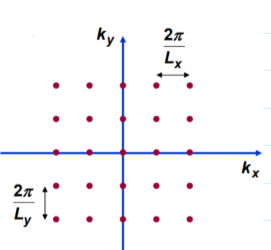
\includegraphics[width=4cm]{Figure/1.png}
    \caption{2-D k space}  
\end{figure}  

\question We can also use plane polar coordinates, $\vec{k}=(|\vec{k}|,\varphi)$, so that $k_{x}=|\vec{k}|\cos\varphi$ and $k_{y}=|\vec{k}|\sin\varphi$ in the standard way. Show that the energy band is a parabola as a function of $k=|\vec{k}|$
\begin{solution}
In the polar coordinates:
\begin{align*}
k_{x} &=|k| \cos \varphi \\
k_{y} &=|k| \sin \varphi \\
\text{So,} E_{k} &=\frac{\hbar^{2}\left(\left|k\right|^{2} \cos ^{2} \varphi+|k|^{2} \sin ^{2} \varphi\right)}{2 m}  \\
&=\frac{\hbar^{2} |\left.k\right|^{2}}{2 m}
\end{align*}
\end{solution}
\newpage
\question  What is the Fermi surface in this 2-dimensional problem ? Please make a drawing in k-space, and mark clearly the occupied and unoccupied regions.
\begin{solution}
The Fermi Surface is when $k_{F}=\sqrt{\frac{2 m E_{F}}{\hbar^{2}}}$, as \textbf{Figure 3} shows, the grid points inside the circle represent the occupied states(yellow part),
while the points outside the circle represent the unoccupied states. 
\end{solution}

\question We must have N electrons confined in our 2-dimensional box. Calculate the electron density $n = \frac{N}{L^{2}}$ using the zero-temperature expression :
\begin{align*}
N=2 \sum_{\vec{k}} \theta\left(k_{F}-|\vec{k}|\right)
\end{align*}
Compare your answer to the analogous law for the 3-dimensional electron gas.
\begin{solution}
Number of electrons is N:
\begin{align*}
N &=2 \sum_{k} \theta\left(k_{F}-|\vec{k}|\right)  \\
&=2 \iint_{|k|<k_{F}} d n_{x}  d n_{y} \\
&=2 \iint \frac{L d k_{x}}{2 \pi} \cdot \frac{L d k_{ y}}{2 \pi} \\
&=\frac{2 A}{(2 \pi)^{2}} \iint d k _{x} d k_{y}  \\
&=\frac{2 A}{(2 \pi)^{2}} \iint d|k|\cdot| k |d \varphi\\
&=\frac{2 A}{(2 \pi)^{2}} \cdot \pi\cdot \left|k_{F}\right|^{2} \\
&=\frac{A}{2 \pi}|k_{F}|^{2}\\
\text{So the electron density is }& n =\frac{N}{A}=\frac{|k_{F}|^2}{2\pi}
\end{align*}
In 3-D case, the Fermi Surface is a sphere, so 
\begin{align*}
N&=2 \iiint d n_{x} d n_{y} dn_{z} \\
&=2  \frac{L^{3}}{(2 \pi)^{3}} \iiint d k_{x} d k_{y} d k_{z} \\
&=\frac{2  L^{3}}{(2 \pi)^{3}} \cdot \frac{4}{3} \pi k_{F}^{3} \\
&=\frac{V}{3 \pi^{2}} k_{F}^{3}\\
\text{The electron density is }& n =\frac{N}{V}=\frac{|k_{F}|^3}{3{\pi}^2}
\end{align*}
\end{solution}
\end{questions}

\end{document}